\begin{frame}{Vanishing/Exploding Gradient}
	\begin{itemize}
		\item The backpropagation algorithm propagates the error gradient while proceeding from the output layer to the input layer. The issue here is the magnitude of the cost function gradients through the layers... 
	\end{itemize}
	\begin{figure}
		\centering
		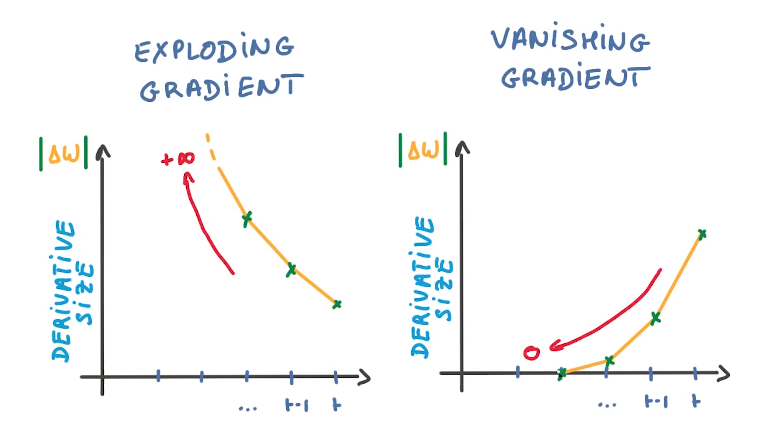
\includegraphics[width=8cm, height=4cm]{Figs/van_2.png}
		\caption{Vanishing/Exploding Gradient, \href{https://medium.com/@ayushch612/vanishing-gradient-and-exploding-gradient-problems-7737c0aa535f}{Source}}
	\end{figure}
\end{frame}

\begin{frame}{Vanishing/Exploding Gradient}
	\begin{itemize}
		\item Vanishing
		\begin{itemize}
			\item Gradients often get smaller as the algorithm progresses down. As a result, gradient descent updates do not effectively change the weights of the lower layer connections, and training never converges.
			\medskip
			\item Make learning slow especially of front layers in the network.
			\medskip
		\end{itemize}
		\item Exploding
		\begin{itemize}
			\item Gradients can get bigger and bigger, so there are very large weight updates at many levels, causing the algorithm to diverge.
			\medskip
			\item The model is not learning much on the training data therefore resulting in a poor loss.
			\medskip
		\end{itemize}
	\end{itemize}
\end{frame}